\subsection{$w_0~w_a$ constraints}

\myparagraph{Method}

In order to assess the impact of the cadence on the cosmological analysis possible with supernovae, we compute the Dark Energy Task force figure of merit \cite{2006astro.ph..9591A} in the Dark Energy parameters $w_0-w_a,$ for a few scenarios. The supernova sample is simulated using (\strech, \sncolor) distributions estimated from \cite{2016ApJ...822L..35S} (High-z G10 parameters) and production rates from  \cite{2008ApJ...682..262D}.

In the first instance, the supernova sample is simulated following roughly the same prescription as that outlined in the recent Science Requirements Document \cite{2018arXiv180901669T}, with small changes to the host redshift selection. For the SRD we adjusted the survey size simulated to ensure roughly 112 000 SNe after host selection cuts from a 4MOST-like ground based telescope. This is the largest determinant of the final size, and so in order to test for differences in the survey strategy we initially doubled the survey size simulated, and then tested a few cadences without requiring any spectrosopic host redshift. This was to ensure that the host-$z$ follow up was not the most important characteristic.
In addition, we imposed a more restrictive cut on the fitted colour in the SAL2T fit from $\sigma(c) < 0.08$ to $\sigma(c) < 0.05.$ Insodoing we are forcing that the supernovae that survive are of higher quality than in the DESC SRD.

In order to test more strongly the impact of the wide field cadence on the overall cosmology, we ran simulations including \textit{only the WFD survey} in addition to a low-$z$ data set. (e.g.  Foundation-like: 2400 \sne~with $z~\less$ 0.1). We compared the cosmology results from the WFD+Foundation surveys for the {\tt kraken\_2026, kraken\_2035} and {\tt altsched, altsched\_rolling} cadences. Finally we show the results with and without spectroscopic host redshift selection for the baseline {\tt kraken\_2026} survey.

We have included only statistical errors: for speed of computation we have neglected the astrophysical systematics. This will be relaxed in future versions.


\begin{figure}[!htbp]
  \begin{center}
  \subfigure[w0-wa ellipses]{\label{fig:w0wa}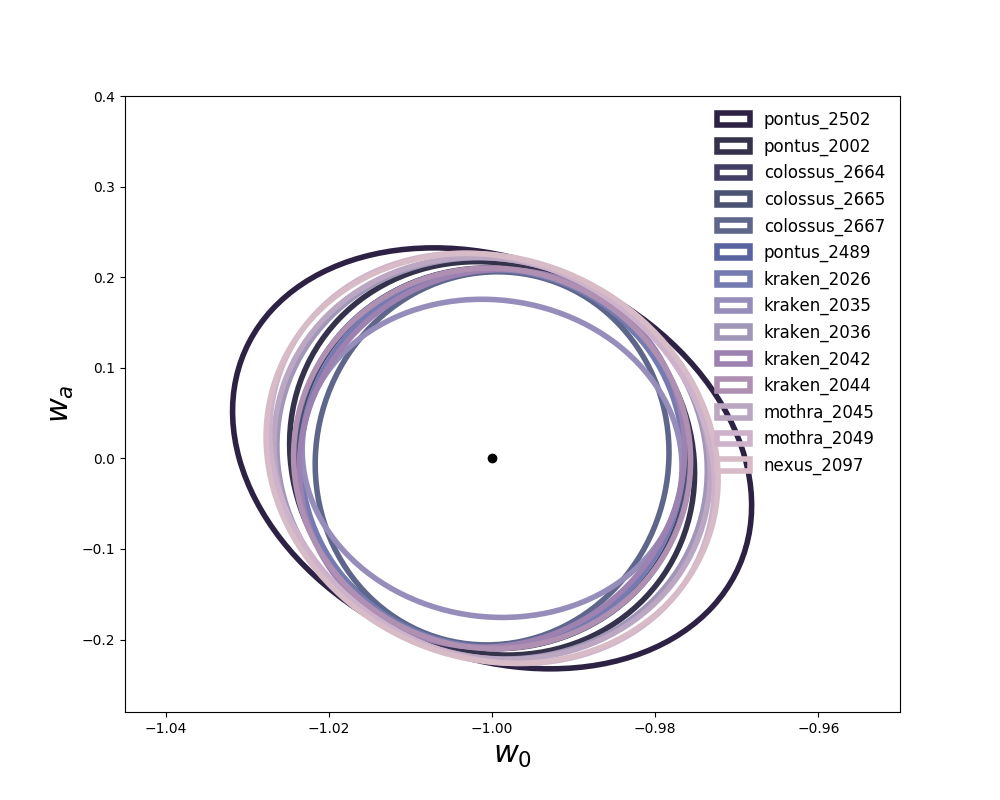
\includegraphics[width=0.7\textwidth]{w0wa/FM_plot_cadence_updated.png}}
    \subfigure[FoM vs observing strategy]{\label{fig:snfom}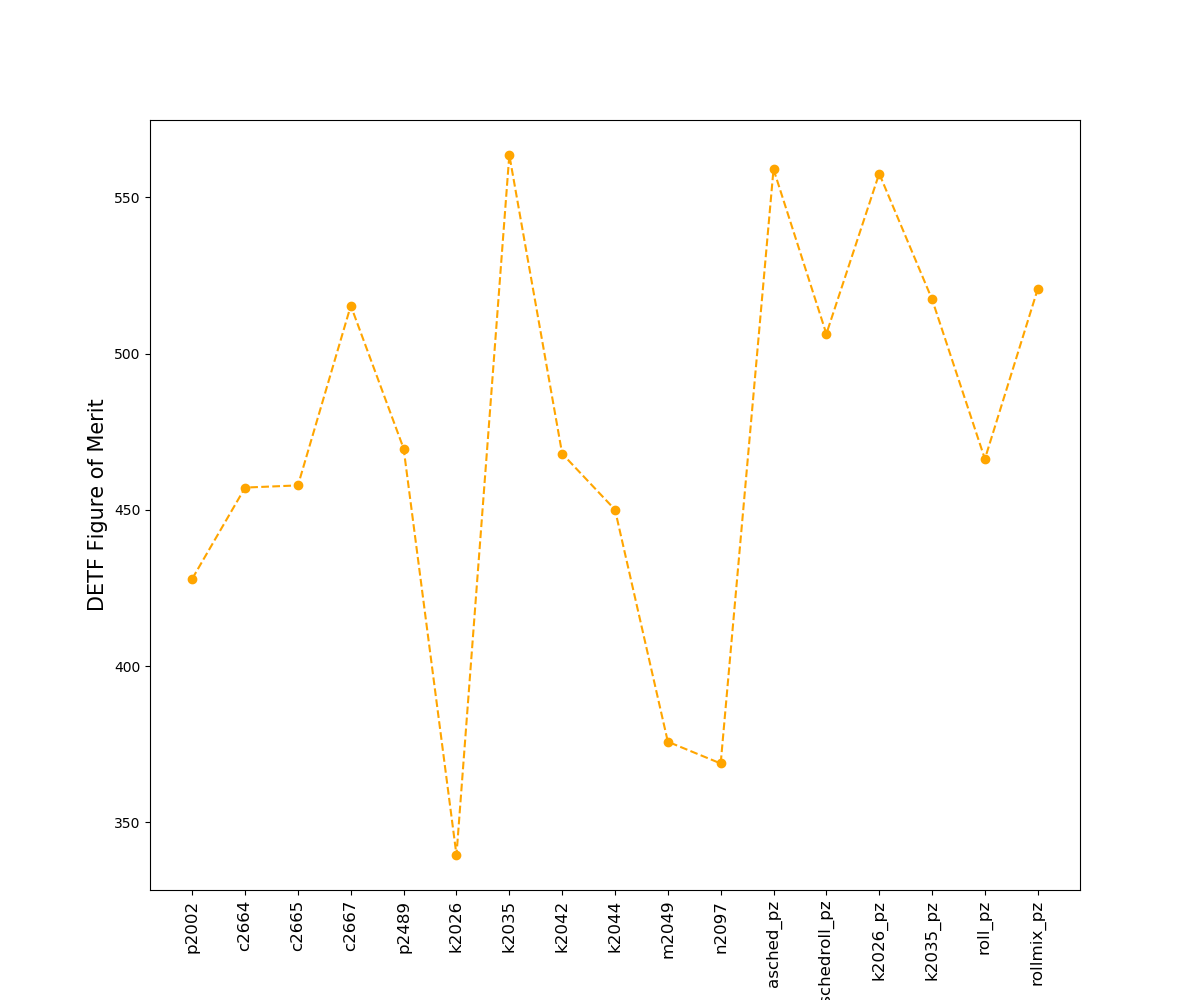
\includegraphics[width=0.7\textwidth]{w0wa/FoM_cadence_updated.png}}
    \caption{Cosmology constraints across cadence types: the ellipses in the $w_0-w_a$ plane (a) and the Dark Energy figure of merit is shown (b) are shown. }
    \end{center}
\end{figure}
\myparagraph{Results}
The largest difference in the Figure of Merit (Fig. \ref{fig:w0wa}) we find is a factor of two between the highest FoM (kraken\_2035) and the lowest FoM (pontus\_2502) if both WDF and DDF surveys are taken into account. The lowest-performing strategy has two alternating bands in declination, switching in alternate years, which is expect to perform poorly. The fact kraken\_2035 is performing better compared to other observing strategies may be explained by the higher number of DD fields observed (9 whereas all other strategies considered 5 fields).

\altsched~ and kraken\_2026 show highest FoMs in WFD-only scenarios (Fig. \ref{fig:snfom}) followed by rolling\_mix, kraken\_2035 , \altsched\_rolling and rolling observing strategies. One may observe that these cadences exhibit the highest FoMs as the following classification shows:
\begin{itemize}
\item{500 $\leq$ FoM}: kraken\_2035, \altsched, kraken\_226, rolling\_mix, kraken\_2035 , \altsched\_rolling and rolling ;
\item{400 $\leq$ FoM $\leq$ 500}: pontus\_2489, kraken\_2042, colossus\_2665, colossus\_2664, kraken\_2044, pontus\_2002 ;
\item{FoM $\leq$ 400}: nexus\_2049, nexus\_2097, kraken\_2026.
\end{itemize}

In the same way as for the number of well-sampled supernovae metric, it is possible to estimate the number of supernovae as a function of the  redshift (observation) limit for \sne~selected to estimate the FoM. The mean redshift is in the range 0.4-0.5 (Fig. \ref{fig:w0wazlim}) and up to 225k supernovae may be collected after ten years of operation.

\begin{figure}[!htbp]
  \begin{center}
    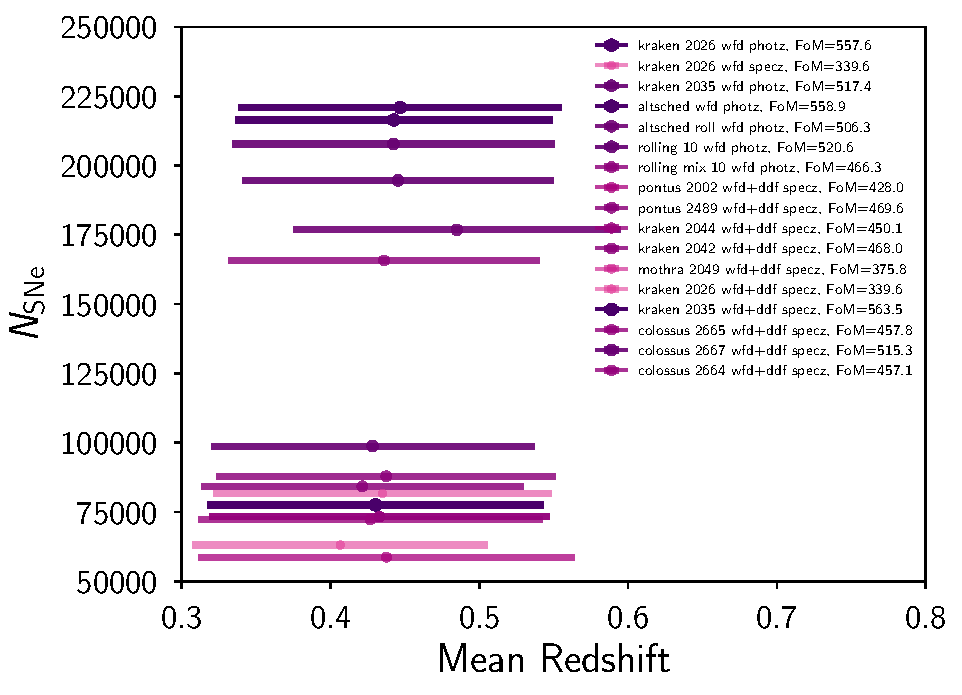
\includegraphics[width=0.8\textwidth]{w0wa/test_numz.pdf}
    \caption{Number of \sne~as a function of the mean redshift. Parameters of the supernovae collected were used as inputs to estimated the FoMs.}
    \label{fig:w0wazlim}
  \end{center}
\end{figure}

A comparison of the deep fields to the WFD for the nominal cadence (kraken\_2026) has shown that the DDF-only survey has about a quarter the number as WFD-only, with mean redshifts of $z~=$ 0.73 and  $z~=$ 0.41 respectively. The DDF survey could enable a competitive dark energy constraint by itself, but two-third of the of the constrainig power will come from WFD: the FoM is equal to 460, 262, 337 for DDF+WFD, DDF, WFD (all +low-$z$) respectively.

\myparagraph{Conclusion}

Even if we may keep in mind that the results presented do not included calibrated (astrophysical) systematics and hence may be optimistic, quite a strong dependence of the FoM values on observing strategies may be noticed: FoM are in the range [340-560] that is a factor 1.6 between the highest and the smallest values. Some of the proposed observing strategies may not be so far to reach the FoM value of 500 (target of the Stage-IV surveys) using supernovae alone.
